\documentclass[12pt,a4paper,twoside,UTF8,fontset=none]{ctexart}

\usepackage[
  top=22mm,
  bottom=26mm,
  inner=26mm,
  outer=22mm,
  headheight=25pt,
  headsep=7mm,
  footskip=12mm
]{geometry}
\usepackage{fontspec}
\usepackage{amsmath,amssymb}
\usepackage[table]{xcolor}
\usepackage{array,booktabs,tabularx,longtable}
\usepackage{hhline}
\usepackage{needspace}
\usepackage{tikz}
\usetikzlibrary{calc}
\usepackage{graphicx}
\usepackage{titlesec}
\usepackage{fancyhdr}
\usepackage{hyperref}
\usepackage{enumitem}
\usepackage{microtype}

\defaultfontfeatures{Ligatures=TeX}
\setmainfont{TeX Gyre Heros}
\setsansfont{TeX Gyre Heros}
\setmonofont{Latin Modern Mono}
\setCJKmainfont[
  Path=./,
  UprightFont=NotoSansSC-Regular.ttf,
  BoldFont=NotoSansSC-Bold.ttf
]{NotoSansSC-Regular.ttf}
\setCJKsansfont[
  Path=./,
  UprightFont=NotoSansSC-Regular.ttf,
  BoldFont=NotoSansSC-Bold.ttf
]{NotoSansSC-Regular.ttf}

\definecolor{GBUBlue}{RGB}{13,0,178}
\colorlet{GBUBlueDark}{GBUBlue!70!black}
\colorlet{GBUBlueLight}{black!3!white}
\colorlet{GBUSessionFill}{black!9!white}
\definecolor{GBUOrange}{RGB}{255,74,5}
\definecolor{GBUPurple}{RGB}{128,0,196}
\definecolor{GBUOchre}{RGB}{164,120,32}
\definecolor{GBUSilver}{RGB}{210,211,207}
\definecolor{GBUBackdrop}{RGB}{245,246,246}
\definecolor{GBUText}{RGB}{0,0,0}
\colorlet{GBURule}{black!45!white}

\hypersetup{
  hidelinks,
  pdfprintscaling=None,
  pdfduplex=DuplexFlipLongEdge,
  pdftitle={2026年秋季组合数学与图论研讨会会议手册（打印版）},
  pdfauthor={大湾区大学理学院}
}

\setlength{\parindent}{2em}
\setlength{\parskip}{0.35em}
\setlength{\emergencystretch}{2em}
\setlength{\arrayrulewidth}{0.5pt}
\setcounter{secnumdepth}{0}
\renewcommand{\baselinestretch}{1.16}
\clubpenalty=10000
\widowpenalty=10000
\displaywidowpenalty=10000
\raggedbottom

\titleformat{\section}
  {\color{GBUBlue}\sffamily\bfseries\Large}
  {}{0pt}{}
  [\vspace{0.25em}{\color{GBUOrange}\titlerule[1.1pt]}]
\titlespacing*{\section}{0pt}{0.8em}{0.9em}

\titleformat{\subsection}
  {\color{GBUBlueDark}\sffamily\bfseries\large}
  {}{0pt}{}
\titlespacing*{\subsection}{0pt}{1.0em}{0.55em}

% The motto and page number are centred on the physical sheet, including
% even pages with mirrored binding margins. The cover and its blank reverse
% remain unnumbered; conference information starts at body page 1.
\newcommand{\printfooter}{%
  \begin{tikzpicture}[remember picture,overlay]
    \node[anchor=base,inner sep=0pt,text=GBUBlue,
      font=\sffamily\fontsize{8}{10}\selectfont]
      at ([yshift=20mm]current page.south)
      {基础扎实、视野开阔、知行合一、融会贯通};
    \node[anchor=base,inner sep=0pt,text=GBUText,
      font=\sffamily\fontsize{9}{11}\selectfont]
      at ([yshift=13mm]current page.south) {\thepage};
  \end{tikzpicture}%
}

\pagestyle{fancy}
\fancyhf{}
\fancyhead[L]{\small\color{GBUBlueDark}2026年秋季组合数学与图论研讨会}
\fancyhead[R]{\small\color{GBUBlueDark}会议手册}
\fancyfoot[C]{\printfooter}
\renewcommand{\headrulewidth}{0.45pt}
\renewcommand{\headrule}{\hbox to\headwidth{\color{GBURule}\leaders\hrule height \headrulewidth\hfill}}
\fancypagestyle{printdivider}{%
  \fancyhf{}
  \fancyfoot[C]{\printfooter}
  \renewcommand{\headrulewidth}{0pt}
  \renewcommand{\headrule}{}
}
\fancypagestyle{plain}{%
  \fancyhf{}
  \fancyfoot[C]{\printfooter}
  \renewcommand{\headrulewidth}{0pt}
  \renewcommand{\headrule}{}
}

\newcolumntype{L}[1]{>{\raggedright\arraybackslash}p{#1}}
\newcolumntype{B}[1]{>{\raggedright\arraybackslash\bfseries\leavevmode\color{GBUBlueDark}}p{#1}}
\newcolumntype{C}[1]{>{\centering\arraybackslash}p{#1}}
\newcolumntype{Y}{>{\raggedright\arraybackslash}X}

\newcommand{\diamondrule}{%
  \begin{center}
    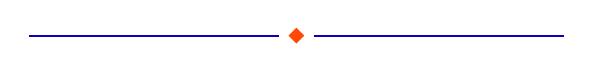
\begin{tikzpicture}
      \draw[GBUBlue, line width=0.7pt] (-3.4,0)--(-0.22,0);
      \fill[GBUOrange] (0,0.10)--(0.10,0)--(0,-0.10)--(-0.10,0)--cycle;
      \draw[GBUBlue, line width=0.7pt] (0.22,0)--(3.4,0);
    \end{tikzpicture}
  \end{center}
}

\newcommand{\sessionrow}[2]{%
  \rowcolor{GBUSessionFill}
  \multicolumn{3}{|c|}{\color{GBUText}\bfseries #1\quad 主持人：#2}\\
  \hhline{|---|}
}

\newcommand{\speakerdisplay}[2]{%
  \textbf{#1}%
  \if\relax\detokenize{#2}\relax
  \else
    \par\vspace{0.04em}{\scriptsize\color{GBUText}#2}%
  \fi
}

\newcommand{\talkrow}[3]{%
  #1 & #2 & #3\\
  \hhline{|---|}
}

\newcommand{\breakrow}[1]{%
  \rowcolor{black!3!white}
  #1 & \multicolumn{2}{c|}{\color{GBUBlueDark}\bfseries 中场休息}\\
  \hhline{|---|}
}

\newenvironment{talkabstract}[3]{%
  \par\addvspace{1.25em}
  \Needspace{13\baselineskip}
  \phantomsection
  \noindent
  \begin{tikzpicture}
    \node[
      anchor=north west,
      text width=\dimexpr\textwidth-0.70cm\relax,
      align=left,
      inner sep=0pt
    ] (talkhead) at (0.45,0) {%
      {\hyphenpenalty=10000\exhyphenpenalty=10000
       \color{GBUBlueDark}\sffamily\bfseries\large #1\par}
      \vspace{0.30em}
      {\sffamily\bfseries 报告人 / Speaker：#2\par}
      \vspace{0.08em}
      {\sffamily\small\color{GBUBlue}单位 / Affiliation：#3\par}
    };
    \fill[GBUBlue]
      ([xshift=-0.45cm]talkhead.north west)
      rectangle
      ([xshift=-0.31cm]talkhead.south west);
  \end{tikzpicture}\par\nobreak
  \vspace{0.25em}
  \noindent{\color{GBUOrange}\rule{\textwidth}{1.0pt}}
  \par\nobreak\vspace{0.20em}

  \noindent{\color{GBUBlue}\sffamily\bfseries 报告摘要 / Abstract}\par
  \small
}{%
  \par\normalsize
  % Do not let a decorative separator become the first item on a new page.
  \ifdim\dimexpr\pagegoal-\pagetotal\relax>3\baselineskip
    \addvspace{0.75em}
    \noindent{\color{GBURule}\rule{\textwidth}{0.45pt}}
    \par\addvspace{0.2em}
  \else
    \addvspace{0.75em}
  \fi
}

\newcommand{\bio}[1]{%
  \par\vspace{0.55em}
  \Needspace{5\baselineskip}
  \noindent{\color{GBUBlue}\sffamily\bfseries 个人简介 / Biography}\par
  \small #1\par
}

\begin{document}
\color{GBUText}
\hypersetup{pageanchor=false}

% --------------------------------------------------------------------------
% Cover: a restrained white layout with the official GBU lockup.
% --------------------------------------------------------------------------
\newgeometry{top=12mm,bottom=15mm,left=20mm,right=20mm}
\thispagestyle{empty}
\thispdfpagelabel{封面}

\begin{center}
  \vspace*{5mm}
  
\includegraphics[width=72mm]{GBU-logo-horizontal-blue.png}\par
  \vspace{13mm}
  {\color{GBUBlueDark}\sffamily\bfseries\fontsize{29}{39}\selectfont
   2026年秋季\\[0.12em]
   组合数学与图论研讨会\par}
  \vspace{5mm}
  {\color{GBUBlue}\sffamily\bfseries\fontsize{17}{22}\selectfont
   会议手册\par}
  \vspace{2mm}
  {\color{GBUBlue}\sffamily\fontsize{10.5}{14}\selectfont
   2026 AUTUMN WORKSHOP ON\\
   COMBINATORICS AND GRAPH THEORY\par}

  \vspace{7mm}
  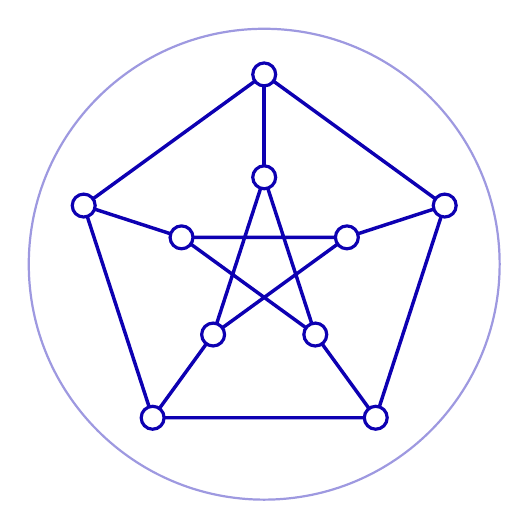
\begin{tikzpicture}[scale=0.92]
    \draw[GBUBlue!40,line width=0.8pt] (0,0) circle (3.25);
    \foreach \i in {1,...,5}{
      \coordinate (o\i) at ({90+72*(\i-1)}:2.62);
      \coordinate (i\i) at ({90+72*(\i-1)}:1.20);
    }
    \draw[GBUBlue,line width=1.25pt]
      (o1)--(o2)--(o3)--(o4)--(o5)--cycle;
    \draw[GBUBlue,line width=1.25pt]
      (i1)--(i3)--(i5)--(i2)--(i4)--cycle;
    \foreach \i in {1,...,5}{
      \draw[GBUBlue,line width=1.25pt] (o\i)--(i\i);
      \fill[white] (o\i) circle (4.5pt);
      \draw[GBUBlue,line width=1.15pt] (o\i) circle (4.5pt);
      \fill[white] (i\i) circle (4.5pt);
      \draw[GBUBlue,line width=1.15pt] (i\i) circle (4.5pt);
    }
  \end{tikzpicture}

  \vspace{5mm}
  \diamondrule
  \vspace{-1mm}
  {\color{GBUBlueDark}\sffamily\bfseries\fontsize{20}{25}\selectfont
   2026年9月4日--6日\par}
  \vspace{1mm}
  {\color{GBUBlue}\sffamily\fontsize{10}{13}\selectfont
   SEPTEMBER 4--6, 2026\par}
  \vspace{6mm}
  {\color{GBUBlueDark}\sffamily\bfseries 主办单位：大湾区大学理学院\par}
\end{center}

\clearpage
\restoregeometry

% Blank inside cover: no header, motto, page number, or other printed marks.
\thispagestyle{empty}
\thispdfpagelabel{空白页}
\null
\clearpage
\pagenumbering{arabic}
\hypersetup{pageanchor=true}
% --------------------------------------------------------------------------
% Conference information
% --------------------------------------------------------------------------
\section{会议概览}

本次研讨会聚焦组合数学、图论及其相关交叉方向，旨在交流最新研究进展，
促进学者之间的深入讨论与合作。

\vspace{0.8em}
\renewcommand{\arraystretch}{1.45}
\arrayrulecolor{GBURule}
\noindent
\begin{tabularx}{\textwidth}{B{3.2cm}Y}
  \toprule
  会议名称 & 2026年秋季组合数学与图论研讨会\\
  英文名称 & 2026 Autumn Workshop on Combinatorics and Graph Theory\\
  会议日期 & 2026年9月4日--6日\\
  报到日期 & 2026年9月4日（具体安排以会务组通知为准）\\
  报告时间 & 9月5日全天、9月6日上午\\
  自由讨论 & 9月6日下午\\
  主办单位 & 大湾区大学理学院\\
  会议地点 & 大湾区大学松山湖校区\\
  具体会场 & 教学楼 B303\\
  住宿酒店 & 湾大松山湖学术交流中心酒店\\
  \bottomrule
\end{tabularx}

\vspace{1.2em}
\noindent
\begin{tikzpicture}
  \fill[GBUBlueLight,rounded corners=3pt] (0,0) rectangle (\textwidth,1.65);
  \fill[GBUOrange] (0,0) rectangle (0.12,1.65);
  \node[
    anchor=west,
    text width=\dimexpr\textwidth-1.0cm\relax,
    align=left
  ] at (0.55,0.82) {%
    \small\color{GBUText}
    报告顺序按报告人姓氏的英文拼写或汉语拼音 A--Z 排列。
    9月5日上午、下午及9月6日上午各安排四场，每场35分钟；
    前两场结束后休息20分钟，随后进行后两场。
  };
\end{tikzpicture}

\vspace{1.0em}
\subsection*{会务组联系方式}
\small
\renewcommand{\arraystretch}{1.45}
\noindent
\begin{tabularx}{\textwidth}{B{2.6cm}Y L{3.6cm}}
  \toprule
  姓名 & \textbf{邮箱} & \textbf{手机}\\
  \midrule
  李伟聪 & \href{mailto:liweicong@gbu.edu.cn}{liweicong@gbu.edu.cn} & \mbox{15267069706}\\
  王靖文 & \href{mailto:wangjw@gbu.edu.cn}{wangjw@gbu.edu.cn} & \mbox{13060696196}\\
  \bottomrule
\end{tabularx}
\normalsize

\clearpage
\renewcommand{\contentsname}{目录}
\setcounter{tocdepth}{1}
{\hyphenpenalty=10000\exhyphenpenalty=10000\sloppy
\tableofcontents}

% --------------------------------------------------------------------------
% Schedule
% --------------------------------------------------------------------------
\clearpage
\section{会议日程 / Schedule}

\subsection{9月5日（星期六）上午}
\noindent\textcolor{GBUBlueDark}{\textbf{开始时间：09:00}}

\vspace{0.45em}
\small
\renewcommand{\arraystretch}{1.38}
\arrayrulecolor{GBURule}
\noindent
\begin{tabularx}{\textwidth}{|C{2.35cm}|C{3.65cm}|Y|}
  \hline
  \rowcolor{GBUBlueLight}
  \textbf{时间} & \textbf{报告人} & \centering\arraybackslash\textbf{报告题目}\\
  \hline
  09:00--09:10 & \multicolumn{2}{c|}{\textbf{开幕式 / Opening}}\\
  \hline
  \sessionrow{第一组报告 / Session 1}{范更华}
  \talkrow{09:10--09:45}{\speakerdisplay{何伟骅}{Weihua HE}}{The Local Average Order of Dominating Sets}
  \talkrow{09:45--10:20}{\speakerdisplay{Ferdinand IHRINGER}{}}{Constructive Ramsey Bounds}
  \breakrow{10:20--10:40}
  \sessionrow{第二组报告 / Session 2}{陆玫}
  \talkrow{10:40--11:15}{\speakerdisplay{季青}{Qing JI}}{Modular Nahm Sums for Symmetrizable Matrices with arbitrary rank}
  \talkrow{11:15--11:50}{\speakerdisplay{毛建玺}{Jianxi MAO}}{The Narayana Transformation}
\end{tabularx}
\normalsize

\vspace{1.4em}
\subsection{9月5日（星期六）下午}
\noindent\textcolor{GBUBlueDark}{\textbf{开始时间：15:00}}

\vspace{0.45em}
\small
\noindent
\begin{tabularx}{\textwidth}{|C{2.35cm}|C{3.65cm}|Y|}
  \hline
  \rowcolor{GBUBlueLight}
  \textbf{时间} & \textbf{报告人} & \centering\arraybackslash\textbf{报告题目}\\
  \hline
  \sessionrow{第一组报告 / Session 1}{王毅}
  \talkrow{15:00--15:35}{\speakerdisplay{王健}{Jian WANG}}{Stability for Helly-type and triangle-free families}
  \talkrow{15:35--16:10}{\speakerdisplay{王六权}{Liuquan WANG}}{Modular Nahm Sums for the Inverse Cartan Matrix of Type $D_r$}
  \breakrow{16:10--16:30}
  \sessionrow{第二组报告 / Session 2}{向青}
  \talkrow{16:30--17:05}{\speakerdisplay{王卫}{Wei WANG}}{Generalized Spectral Characterizations Under Graph Operations}
  \talkrow{17:05--17:40}{\speakerdisplay{向子卿}{Ziqing XIANG}}{Permutation automorphism groups of random cyclic codes}
\end{tabularx}
\normalsize

\clearpage
\section*{会议日程 / Schedule（续）}

\subsection{9月6日（星期日）上午}
\noindent\textcolor{GBUBlueDark}{\textbf{开始时间：09:00}}

\vspace{0.45em}
\small
\noindent
\begin{tabularx}{\textwidth}{|C{2.35cm}|C{3.65cm}|Y|}
  \hline
  \rowcolor{GBUBlueLight}
  \textbf{时间} & \textbf{报告人} & \centering\arraybackslash\textbf{报告题目}\\
  \hline
  \sessionrow{第一组报告 / Session 1}{周胜林}
  \talkrow{09:00--09:35}{\speakerdisplay{徐子翔}{Zixiang XU}}{Three conjectures on Sperner families}
  \talkrow{09:35--10:10}{\speakerdisplay{杨立波}{Libo YANG}}{Hadamard product and interlacing symmetric decomposition}
  \breakrow{10:10--10:30}
  \sessionrow{第二组报告 / Session 2}{周正春}
  \talkrow{10:30--11:05}{\speakerdisplay{叶智恺}{Chi Hoi YIP}}{Ill-distributed Sidon sets}
  \talkrow{11:05--11:40}{\speakerdisplay{张华军}{Huajun ZHANG}}{On intersecting families with covering number $3$}
\end{tabularx}
\normalsize

\vspace{1.2em}
\noindent\small\color{GBUText}
说明：会场为教学楼 B303；六位主持人按姓氏拼音顺序依次主持各组报告。
\normalsize

\vspace{1.2em}
\subsection{9月6日（星期日）下午}
\noindent
\begin{tikzpicture}
  \fill[GBUBlueLight,rounded corners=3pt] (0,0) rectangle (\textwidth,1.35);
  \fill[GBUOrange] (0,0) rectangle (0.12,1.35);
  \node[anchor=west,text=GBUBlueDark,font=\sffamily\bfseries\large]
    at (0.55,0.68) {自由讨论 / Open Discussion};
\end{tikzpicture}

% --------------------------------------------------------------------------
% Abstracts: titles and abstracts are preserved from the submitted sources.
% --------------------------------------------------------------------------
\clearpage
\phantomsection
\addcontentsline{toc}{section}{报告摘要 / Abstracts}
% White divider page avoids a full-page colour background in print.
\begin{center}
  \vspace*{23mm}
  
\includegraphics[width=58mm]{GBU-logo-horizontal-blue.png}\par
  \vspace{12mm}
  {\color{GBUBlueDark}\sffamily\bfseries\fontsize{30}{38}\selectfont
   报告摘要\par}
  \vspace{2mm}
  {\color{GBUBlue}\sffamily\fontsize{16}{21}\selectfont
   ABSTRACTS\par}
  \vspace{9mm}
  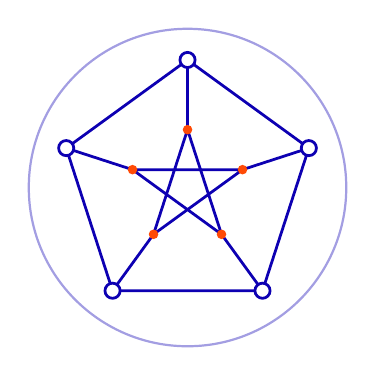
\begin{tikzpicture}[scale=0.72]
    \draw[GBUBlue!38,line width=0.8pt] (0,0) circle (2.8);
    \foreach \i in {1,...,5}{
      \coordinate (a\i) at ({90+72*(\i-1)}:2.25);
      \coordinate (b\i) at ({90+72*(\i-1)}:1.02);
    }
    \draw[GBUBlue,line width=1.0pt] (a1)--(a2)--(a3)--(a4)--(a5)--cycle;
    \draw[GBUBlue,line width=1.0pt] (b1)--(b3)--(b5)--(b2)--(b4)--cycle;
    \foreach \i in {1,...,5}{
      \draw[GBUBlue,line width=1.0pt] (a\i)--(b\i);
      \fill[white] (a\i) circle (3.8pt);
      \draw[GBUBlue,line width=1.0pt] (a\i) circle (3.8pt);
      \fill[GBUOrange] (b\i) circle (2.4pt);
    }
  \end{tikzpicture}
  \vfill
  {\color{GBUBlueDark}\sffamily 报告人按姓氏 A--Z 排列\par}
\end{center}
\thispagestyle{printdivider}
\clearpage

\begin{talkabstract}
  {The Local Average Order of Dominating Sets}
  {何伟骅（Weihua HE）}
  {广东工业大学}
We conduct a systematic study on the average order of dominating sets containing a fixed vertex and show that the average order of dominating sets containing a fixed vertex $v$ of a graph with $n$ vertices is at least $\frac{n+1}{2}$, with this lower bound achieved when $v$ is adjacent to all other vertices in the graph. Furthermore, for a graph on $n$ vertices without isolated vertices, we show that $\frac{5n+2}{6}$ is an upper bound for the average order of dominating sets containing a fixed vertex. Moreover, we derive a formula for the average order of dominating sets containing a fixed vertex in the case where the degree of the fixed vertex is $n-2$, and determine an upper bound of $\frac{4n+1}{6}$ for a $l$-stem when $l \geq 2$.

\bio{何伟骅，教授，硕士生导师，广东工业大学数学与统计学院副院长，2008年本科毕业于中国科学技术大学，2014年博士毕业于法国巴黎第十一大学（现更名为巴黎萨克雷大学），主要从事图论及其应用、算法、机器学习的研究工作。}
\end{talkabstract}

\begin{talkabstract}
  {Constructive Ramsey Bounds}
  {Ferdinand IHRINGER}
  {南方科技大学}
For Ramsey numbers $R(s, t)$, it is very easy to find good probabilistic
constructions, but seemingly very hard to find explicit constructions.
We give a construction showing that, uniformly for
integers $3 \leq s \leq t$, as $t \to \infty$, \[
R( s,t ) \geq t^{(1-o(1)) \log s / \log(\log s + 1) }. \]
For fixed $s$, this improves the dependence on $s$ in the general off-diagonal
construction of Alon and Pudl\'ak. In particular, $R(33, t) \geq t^{2.1-o(1)}$,
to our knowledge, the first explicit construction showing $R(s, t) \geq t^c$
for some fixed $s$ and some $c > 2$. In the diagonal case, it improves the
leading constant in the exponent of the classical Frankl--Wilson bound.

\bio{Ferdinand IHRINGER（伊林格），南方科技大学数学系助理教授，2015年博士毕业于德国吉森大学（Justus-Liebig-Universität Gießen），导师为 Klaus Metsch。主要研究领域包括极值组合、有限几何、图谱理论以及编码理论等，在 Combinatorica、Journal of Combinatorial Theory A、Journal of Combinatorial Theory B、Proceedings of the American Mathematical Society 等杂志发表论文多篇。}
\end{talkabstract}

\begin{talkabstract}
  {Modular Nahm Sums for Symmetrizable Matrices with arbitrary rank}
  {季青（Qing JI）}
  {天津大学}
Recently, we construct three families of modular Nahm sums for symmetrizable matrices with arbitrary rank $r\geq 2$ of indices $({2,\ldots, 2},1)$ and $({1,\ldots, 1},2)$. The cases $r = 2$ and $r = 3$ of these families were previously established by Mizuno, Warnaar, and B. Wang--L. Wang. Building upon these three families, we construct two vector-valued automorphic forms, one of which is a vector-valued modular function when $r$ is odd. The problem is whether the remaining components of these two vector-valued automorphic forms can be expressed as linear combinations of Nahm sums for symmetrizable matrices. This work is joint with Julia Q. D. Du (杜庆丹), Erin Y. Y. Shen (沈一颖) and Clara X. Y. Xu (许晓瑜). 

\bio{季青，天津大学国家应用数学中心教授，国家优青获得者。主要从事组合数学的研究，解决了沃尔夫奖获得者和多位美国科学院院士提出的猜想和公开问题，相关成果发表在包括 J. Reine Angew. Math.、Adv. Math.（3篇）、Trans. Amer. Math. Soc.（2篇）、J. Combin. Theory A（3篇）等期刊上，并被多位著名学者在包括权威杂志 Notice AMS 上正面引用。多次主持国家自然科学基金项目，参与国家自然科学基金委的创新群体项目和重点项目。}
\end{talkabstract}

\begin{talkabstract}
  {The Narayana Transformation}
  {毛建玺（Jianxi MAO）}
  {大连理工大学}
For $m\in\mathbb{Z}_{\geq 0}$, let $$N_{n,m}(x)={}_2F_1(-n,-n-m;m+1;x),$$
which specializes to the Narayana polynomials of types $B$ and $A$ for $m=0$ and $m=1$, respectively. We prove that the associated basis transformation
$$T_{N_m}\left(\sum_{k=0}^n a_kx^k\right)=\sum_{k=0}^n a_kN_{k,m}(x)$$
maps every real-rooted polynomial with nonnegative coefficients to a real-rooted polynomial. The proof is based on the rectangular additive convolution of polynomials. We then apply this result to products of lower triangular matrices and obtain a general criterion ensuring that their row generating functions remain real-rooted. As consequences, we recover this property for powers and products of several classical triangular matrices, including Pascal's triangle, the Stirling triangles, and the Narayana triangles of types $A$ and $B$. We conclude with conjectures concerning the squares of the Eulerian and Delannoy triangles.

\bio{毛建玺，大连理工大学副教授。2021年毕业于大连理工大学，获理学博士学位，研究方向为组合数学。主要研究兴趣包括解析组合学和计数组合学。在组合数学领域主流期刊发表论文十余篇。主持国家自然科学基金青年项目，主持完成中国博士后面上基金项目。}
\end{talkabstract}

\begin{talkabstract}
  {Stability for Helly-type and triangle-free families}
  {王健（Jian WANG）}
  {四川大学}
The $k$-graph $\mathcal{F}$ is called Helly if all its intersecting subfamilies are stars. In 1984 Tuza proved the best possible bound $|\mathcal{F}|\leq \binom{n-k-1}{k-1}+\binom{n-2}{k-2}+1$ for Helly families that are not stars for some unspecified $n>n_0(k)$. Recently, we establish the same bound for the full range $n\geq 2k$. We also show that for $n>12k^2$ the same upper bound holds for triangle-free families. Joint work with Peter Frankl.

\bio{王健，2016年获南开大学应用数学博士学位，导师为陈永川院士。主要研究极值组合学与极值集合论，关注相交集族、超图匹配、超图图兰问题及其稳定性。}
\end{talkabstract}

\begin{talkabstract}
  {Modular Nahm Sums for the Inverse Cartan Matrix of Type $D_r$}
  {王六权（Liuquan WANG）}
  {武汉大学}
For $r\geq 3$ we denote by $\mathcal{C}(D_r)$ the Cartan matrix of type $D_r$. Recently, Sun and Wang conjectured a Rogers--Ramanujan type identity for the Nahm sum associated with $\mathcal{C}(D_r)^{-1}$ and the zero vector. They further conjecture that there exist $r-1$ companion modular Nahm sums associated with nonzero vectors. We partially prove this conjecture by constructing $\lfloor (r+4)/2\rfloor$ modular Nahm sums for $\mathcal{C}(D_r)^{-1}$. To prove their modularity, we utilize the method of Bailey pairs to establish various Rogers--Ramanujan type identities. In particular, we confirm their conjectural identity. This talk is based on a joint work with Shangwen Wang (王尚文).

\bio{王六权，武汉大学数学与统计学院教授，主要从事组合数学与数论领域的研究，研究课题多集中在 \(q\)-级数、整数分拆、特殊函数、模形式理论等方面。迄今在《Advances in Mathematics》、《Transactions of the American Mathematical Society》、《Journal of Combinatorial Theory Series A》、《Advances in Applied Mathematics》、《Journal of Number Theory》等期刊上发表学术论文50多篇，先后主持国家自然科学基金青年基金、面上项目、国家重点研发计划青年科学家项目各一项。}
\end{talkabstract}

\begin{talkabstract}
  {Generalized Spectral Characterizations Under Graph Operations}
  {王卫（Wei WANG）}
  {西安交通大学}
A graph G is determined by its generalized spectrum if for any graph H, whenever H is cospectral with G and their complements are also cospectral, then H is isomorphic to G. In this talk, we present some recent results concerning the generalized spectral determination of graphs constructed via graph operations including line graphs, subdivision graphs, and others.

\bio{王卫，西安交通大学数学与统计学院教授、博士生导师。主要研究领域为代数图论与组合最优化。在图谱理论的研究中对图的广义谱刻画问题做出了一些原创性的工作，在组合优化领域中对一些 NP-困难组合优化问题设计出了一些好的近似算法。在 J. Combin. Theory, Ser B、European J. Combin. 以及 IEEE/ACM Transactions 系列等组合图论刊物上发表研究论文80余篇，主持（完成）国家自然科学基金面上项目多项。目前担任中国运筹学会图论与组合分会常务理事、陕西省工业与应用数学学会理事长及国际 SCI 期刊 \emph{Linear Algebra Appl.}、\emph{Discrete Mathematics, Algorithms and Applications} 编委等。}
\end{talkabstract}

\begin{talkabstract}
  {Permutation automorphism groups of random cyclic codes}
  {向子卿（Ziqing XIANG）}
  {南方科技大学}
In 1998, Berger-Charpin conjectured that the permutation automorphism groups of random cyclic codes are generated by shifting and Frobenius on the coordinates. There are many positive results on this conjecture. In 2010, Bienert-Klopsch proved the conjecture when length is prime, and in 2026, Feng-Hollmann-Li-Xiang proved the conjecture for random nondegenerate irreducible cyclic codes. In this talk, we will show that this group is actually not the correct expected automorphism group, and we will give a refined version of the conjecture. We will also discuss a systematical way to study the automorphism group. This is joint work with Yanni Wu.

\bio{向子卿，南方科技大学数学系兼深圳国家应用数学中心副教授、博士生导师，国家级青年人才，2022年国际组合数学及其应用协会 Kirkman 奖章获得者。他于2014年本科毕业于上海交通大学，2019年获得美国佐治亚大学数学博士学位。他的研究兴趣主要集中在代数组合和表示论，研究成果发表在 Advances in Mathematics、Journal of Combinatorial Theory A、Journal of Algebraic Combinatorics、Transformation Groups 等期刊上。}
\end{talkabstract}

\begin{talkabstract}
  {Three conjectures on Sperner families}
  {徐子翔（Zixiang XU）}
  {浙江大学}
Sperner families are antichains in the Boolean lattice and have become fundamental objects in the field of combinatorics. In this talk, I will introduce three conjectures concerning Sperner families and discuss recent progress on them.

\bio{徐子翔，浙江大学数学科学学院百人计划研究员。2022 年于首都师范大学获得理学博士学位，导师为葛根年教授。2022 年 9 月至 2026 年 5 月于韩国基础科学研究院极值组合与概率组先后任博士后研究员、高级研究员，合作导师为刘鸿教授。目前的研究方向主要为极值组合以及相关领域如离散几何、信息科学等。已在 Sci. China Math.、IMRN、Israel J. Math.、Combinatorica、JCTA、SIDMA、IEEE TIT 等期刊发表学术论文 20 余篇。}
\end{talkabstract}

\begin{talkabstract}
  {Hadamard product and interlacing symmetric decomposition}
  {杨立波（Libo YANG）}
  {南开大学}
Athanasiadis, Douvropoulos, and Kalampogia-Evangelinou proved that the $h$-polynomial of the order complex of the noncrossing partition lattice of a finite Coxeter group $W$ of rank $r_W$ has a nonnegative real-rooted symmetric decomposition with respect to $r_W-1$. Recently, Alice Gao, Xin-Bei Liu, James Zhao, and I strengthened this result to an interlacing symmetric decomposition and generalized it to $k$-divisible noncrossing partition posets. In this talk, we will discuss some general machinery for proving interlacing symmetric decompositions using the Hadamard product.

\bio{杨立波，南开大学教授，博士生导师。现任南开大学组合数学中心副主任。1999年毕业于郑州大学，获理学学士学位。2004年毕业于南开大学，获理学博士学位。杨立波教授主要从事组合数学方面的研究，特别是对称函数理论和单峰型理论方面，解决了包括美国科学院院士Richard Stanley教授提出的zrank猜想在内的多个公开问题。杨立波教授的成果已在《Trans. Amer. Math. Soc.》、《Intern. Math. Res. Notices》、《J. Combinatorial Theory Series, A》、《Adv. Appl. Math.》、《SIAM Discrete Math.》等重要数学期刊发表学术论文40余篇。2011年入选教育部新世纪优秀人才支持计划，主持过多个国家自然科学基金项目，包括优秀青年科学基金和杰出青年科学基金项目。}
\end{talkabstract}

\begin{talkabstract}
  {Ill-distributed Sidon sets}
  {叶智恺（Chi Hoi YIP）}
  {香港科技大学}
It is known that near-extremal Sidon sets \(A\subseteq [N]\), with \(|A|\geq (1-o(1))N^{1/2}\), must be well distributed. In this talk, I will discuss a converse phenomenon for ill-distributed Sidon sets. Making progress on a question of Alon and Erd\H{o}s, I will show that if \(A\subseteq [N]\cap S\) is a Sidon set, where \(S\) denotes the set of perfect squares, then
\[
|A|\leq \sqrt{N}\exp\left(-c\frac{\log N}{\log\log N}\right)
\]
for some absolute constant \(c>0\). I will also explain how a similar method leads to new bounds for a question of Erd\H{o}s and Guy on point sets in the grid \([N]\times [N]\) with no repeated distances. Joint work with Ernie Croot, Junzhe Mao, Cosmin Pohoata, and Adam Sheffer.

\bio{叶智恺（Chi Hoi YIP），香港科技大学数学系助理教授。2024年获加拿大英属哥伦比亚大学数学博士学位，后任美国佐治亚理工学院 Hale Visiting Assistant Professor。主要研究算术组合及其与解析数论、丢番图方程、极值组合和有限几何的联系。}
\end{talkabstract}

\begin{talkabstract}
  {On intersecting families with covering number $3$}
  {张华军（Huajun ZHANG）}
  {绍兴大学}
The covering number of a family $\mathcal{F}$ is the size of the smallest set that intersects every set in the family, denoted by $\tau(\mathcal{F})$.
For $1 \leq p \leq k-2$, define
\[
\mathcal{B}_p = \{[2,k] \cup \{j\} : k+1 \leq j \leq k+p+1\} \cup \{[k+1, 2k]\},
\]
\[
\mathcal{A}_p = \left\{ A \in \binom{[n]}{k} : 1 \in A, \text{ and } A \cap B \neq \emptyset \text{ for each } B \in \mathcal{B}_p \right\}
\]
and
\[
\mathcal{G}_p(n,k) = \mathcal{A}_p \cup \mathcal{B}_p.
\]
In this talk, we prove that for $n > 2k$ and $k \geq 4$, if $\mathcal{F}$ is a maximal intersecting family in $\binom{[n]}{k}$ with $\tau(\mathcal{F}) \geq 3$ and
\[
|\mathcal{F}| \geq |\mathcal{G}_2(n,k)|,
\]
then $\mathcal{F} \cong \mathcal{G}_1(n,k)$ or $\mathcal{F} \cong \mathcal{G}_2(n,k)$.
This generalizes the results obtained by Kupavskii, Frankl and Wang, respectively.

\bio{张华军，绍兴大学教授，浙江省高校中青年学科带头人，中国组合数学与图论专业委员会委员。主要从事组合极值理论研究，解决了该领域中的多个公开问题与猜想，多篇论文发表在组合数学与图论领域的国际权威期刊J. Combin.Theory Ser. A、J. Combin.Theory Ser. B、J.Graph Theory和SIAM J. Discrete Math.，部分结果已被多本国内外专著作为主要定理收录，主持或完成国家自然科学基金多项。}
\end{talkabstract}

% --------------------------------------------------------------------------
% Transport information: concise, text-only, no map image.
% --------------------------------------------------------------------------
\clearpage
\section{交通信息 / Transportation}

\noindent
\textbf{\color{GBUBlueDark}会议地点：}
大湾区大学松山湖校区教学楼 B303（广东省东莞市松山湖高新技术产业开发区大学路16号）。

\noindent
\textbf{\color{GBUBlueDark}住宿酒店：}
湾大松山湖学术交流中心酒店。

\vspace{0.8em}
\small
\renewcommand{\arraystretch}{1.42}
\noindent
\begin{tabularx}{\textwidth}{B{3.2cm}Y L{3.1cm}}
  \toprule
  到达点 & 推荐方式 & 平峰参考车程\\
  \midrule
  深圳宝安机场 &
  建议乘出租车或网约车直达学校；也可提前核实机场至东莞松山湖候机楼的公共客运班线。 &
  约50--75分钟\\
  虎门站 &
  高铁出行建议优先选择；抵站后可乘地铁或\mbox{快捷巴士}前往大湾区大学（松山湖校区），也可乘出租车或网约车直达学校。 &
  约35--50分钟\\
  松山湖北站 &
  城际铁路出行建议优先选择，抵站后乘出租车或网约车到校。 &
  约15--25分钟\\
  \bottomrule
\end{tabularx}
\normalsize

\vspace{1em}
\noindent
\begin{tikzpicture}
  \fill[GBUBlueLight,rounded corners=3pt] (0,0) rectangle (\textwidth,2.2);
  \fill[GBUOrange] (0,0) rectangle (0.12,2.2);
  \node[
    anchor=west,
    text width=\dimexpr\textwidth-1.0cm\relax,
    align=left
  ] at (0.55,1.1) {%
    \small\color{GBUText}
    出发当日请使用地图软件导航至“大湾区大学（松山湖校区）”。
    以上车程为通常路况下的参考区间，早晚高峰、节假日及恶劣天气可能明显延长；
    铁路和客运班次请以12306、广东城际及深圳机场当日信息为准。
  };
\end{tikzpicture}

\vfill
\diamondrule
\begin{center}
  {\color{GBUBlueDark}\sffamily\bfseries
  欢迎来到大湾区大学}
\end{center}

% --------------------------------------------------------------------------
% Campus guide: preserve the supplied map; give building-level directions
% without inventing an indoor position or an unverified walking route.
% --------------------------------------------------------------------------
\clearpage
\section{校园导览 / Campus Guide}

\noindent
请先在图中找到“教学楼”和“学术交流中心”，分别对应本次会议的会场和住宿地点。

\vspace{0.7em}
\noindent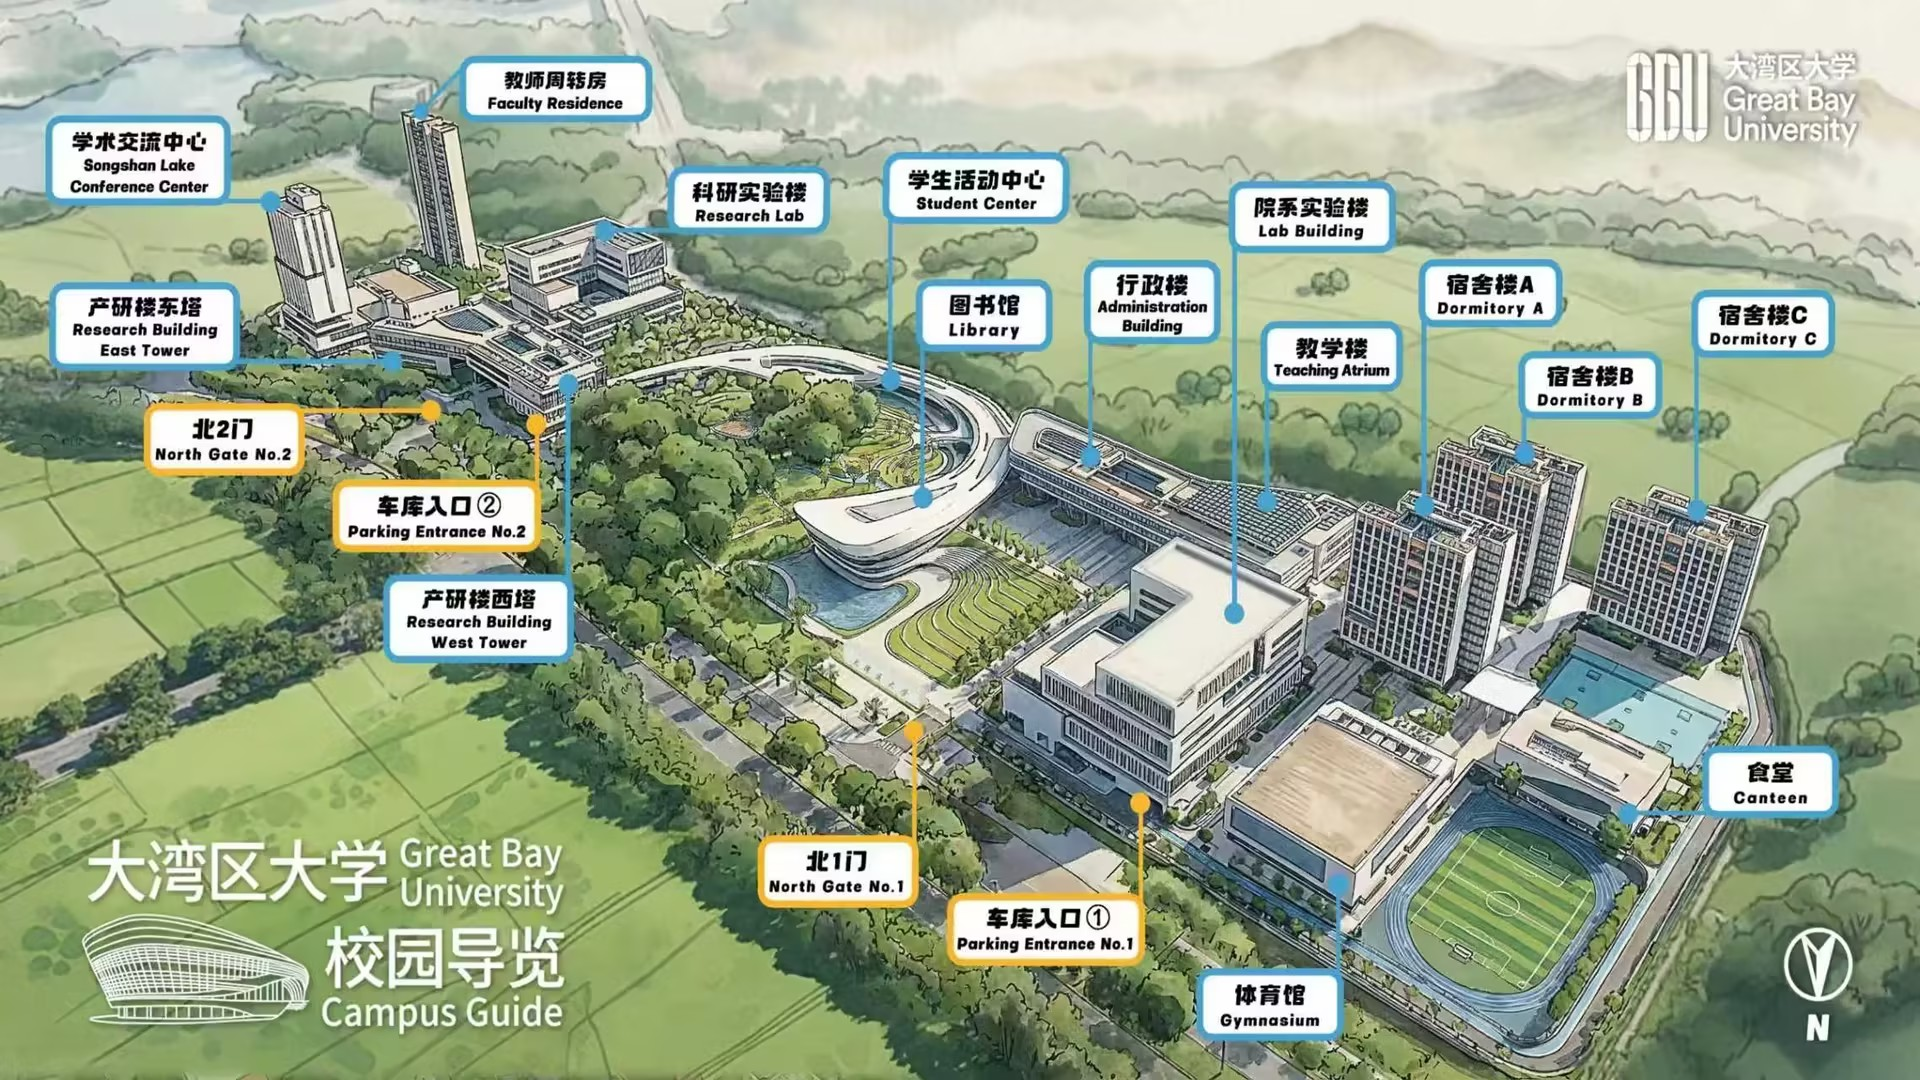
\includegraphics[width=\textwidth]{GBU-campus-guide.jpg}

\vspace{1.0em}
\subsection*{会场与住宿指引}
\renewcommand{\arraystretch}{1.4}
\small
\noindent
\begin{tabularx}{\textwidth}{B{2.0cm}Y}
  \toprule
  会场 & \textbf{教学楼 B303}\\
       & 对应图中“教学楼 / Teaching Atrium”（图中部偏右）。进入教学楼后，请按楼内导视前往 B303；本图不标注具体教室位置。\\
  \midrule
  住宿 & \textbf{湾大松山湖学术交流中心酒店}\\
       & 对应图中“学术交流中心 / Songshan Lake Conference Center”（图左上方）。\\
  \midrule
  入校 & 图中已标明北1门、北2门及车库入口。请按会务通知和学校现场指引入校。\\
  \bottomrule
\end{tabularx}
\normalsize

\vspace{0.8em}
\noindent\small
本图用于校园建筑定位，实际通行路线及楼内位置请以现场导视为准。
\normalsize

\end{document}
